\documentclass[11pt]{beamer}
\usetheme{CambridgeUS}
\usepackage[utf8]{inputenc}
\usepackage{amsmath}
\usepackage{amsfonts}
\usepackage{amssymb}
\usepackage[T1]{fontenc}
\usepackage[utf8]{inputenc}

\author{Rubens Figueiredo}
\title{WIP: Baseboxes}
\setbeamercovered{transparent} 
\setbeamertemplate{navigation symbols}{}
%\logo{} 
\institute{BISDN GmbH} 
\date{\today} 
\subject{Switching devices in Software-Defined Networking} 

\begin{document}

\begin{frame}
\titlepage
\end{frame}

\begin{frame}
\tableofcontents
\end{frame}

% In the past decade Open Networking and Open       
% Disaggregated hardware software architectures have 
% gained prominence.
% => Talk about SDN, what is the connection between SDN and OpenNetworking
% => How open networking is an essential step to enable SDN in the datacenter

% Network Operating Systems(NOS) based 
% on Linux-native hardware offload for network switching 
% ASICs have gained traction.
% => What do we gain by designing our own distro; what are the disadvanatges; 
% => OpenFlow role in offloading the Netlink events

% Linux-native kernel 
% networking hardware offload model has a big advantage 
% in its ability to leverage the tooling ecosystem that 
% already exists and is well understood in the Linux 
% community.
% => tooling ecosystem; Yocto fits here;
% => Speak about GNU Guix, 

% Some of the benefits include: Open Linux firmware management,
% platform driver infrastructure
% => vendor specific drivers; forward porting necessary for many necessary features
%	=> Give example of VxLAN backporting, sucess stories
% => lack of a centralized repo for driver specific components; we must strive for mainlining
% network interface management,
% => Tap interfaces as an abstraction for physical ports; what where the limitations we found while using tap drivers
% => Weaknesses in Tap interfaces as abstracted model:	
% 	=> Statistics mismatch, 
%	=> Unable to correctly represent network state
%	=> State is default UNKOWN
% => Pros in using Tap interfaces:
%	=> ease of configuration
%	=> ease of running everywhere, **find useful architecture for remote switch management
%	=> offswitch/onswitch architecture
% variety of Linux tools 
% => Case study of how does Basebox natively interacts with other Linux tools
%	=> FRR: BGP and OSPF route establishment; mention interop with ECMP Vxlan, talk about necessary adaptations to make it work
%		=> In short, the lack of in kernel support for arp surpression made it necessary to implement own solution to snoop on bridge fdb.
%	=> native radvd
%	=> systemd-networkd as a source for persitent configuration.
%	=> iproute2. **show video on basic setup, bridging.
% and of course a well established ecosystem and community.
% => Mention again Yocto.

% Recently announced project DENT [1] is one another step 
% in the right direction that leverages Linux-native 
% kernel networking and brings together switch ASIC 
% vendors, distributors, system integrators and users.
% => Possibility of creating platform specific repo, what can we possibly propose to how to drive discussion
% 
% This workshop is similar to previous netdevconf 
% switchdev workshops with a larger focus on community 
% discussions around building an Open Linux kernel 
% switchdev based Network Operating System.
% 
% Workshop topics (Work in progress):
% 
% - Discuss switchdev driver updates since last 
%   netdev0x13:
% 
%   - Mellanox mlxsw driver updates
% 
% - New Networking features and use-cases
% 
% - Open issues and challenges
% 
% - New vendors
% 
% - Supporting new features down the pike:
% 
%   - Eg: EVPN-MH, port security, dynamic NAT and others
% 
% - Operationalizing Linux networking:
% 
%   - Automation and DevOps
% 
% [1] linuxfoundation.org press release: dent launches to simplify...


% 
% What is the story? 
% 	Since Software-Defined Networking began as an idea, through procotols like OpenFlow, it changed the landscape of networking.
%	Through benefits like Control-Dataplane separation, which, while present before **find example** it suddenly made a lot more sense to support this type of network role division.

%	baseboxd has evolved throught the years from being a full blown SDN controller, to being "just" the switch agent.
%	It is currently the main source of communication between user and Kernel space in BISDN Linux, our Yocto based Network Operating System.

%	We are currently releasing BISDN Linux with native support for FRR, systemd-networkd, iproute2, and other common Linux tools, which allows us for less investment needed to write own software. Also extremely easy to support for new tools, we are moving all platforms to recent kernels, so we are up to date with recent patches. Although we are still at FRR 6.0.

%	baseboxd "speaks" Netlink northboud, and southbound via Openflow to the OpenFlow Data Path Abstraction, a.k.a OFDPA. By adapting the Netlink system calls to the OpenFlow data model we are able to represent networking state in Linux, currently supporting L2 bridging, L3 static routing, routing protocols like BGP and OSPF though FRRouting, and some initial VxLAN implementation.

% How does baseboxd work?

% Northbound

%	Bound to the Netlink socket, we subscribe to the Netlink events, and listen to the following messages:
%		=> RTM_NEWLINK; RTM_DELLINK; RTM_GETLINK
%		=> RTM_NEWNEIGH; RTM_DELNEIGH; RTM_GETNEIGH
%		=> RTM_NEWROUTE; RTM_DELROUTE; RTM_GETROUTE
%		=> RTM_NEWADDR; RTM_DELADDR; RTM_GETADDR

% 	Each of these messages are associated with rtnetlink. rtnetlink is a part of Netlink, a interface between userspace and the Linux Kernel, allowing the user to do **new, **get and **del operations on networking devices inside the kernel. Employing Netlink are applications like iproute2 and FRR. This interface replaces the more traditional ioctl calls.

% Start speaking about caching mechanism
% 

% Southbound

%	baseboxd then translates the information carried by the previously mentioned messages into the OpenFlow datamodel. BISDN has previously implemented OpenFlow help libraries, which we leverage for communication with OFPDA/ofagent, which are two Broadcom OpenFlow daemons, which then interact with the ASIC's SDK. 
%	rofl: Revised OpenFlow library
%		rofl-common: Standard OpenFlow library, supporting OpenFlow versions from **check
%		rofl-ofdpa: OpenFlow library designed to work with the TableType Patterns present in the OFDPA implementation.

% 	We also respond to switch events triggered from the ASIC. We currently handle port state and OpenFlow error messages.
 

% How did the story develop?figure

% Goals
% 	Run a Linux Based Operating system on whiteboxed networking devices;
% 	
% Desired System
% 	Configuration flexibility, we want people to feel as familiar as possible;
% 	Interoperability between other networking devices => obvious
% 			
% Property Analysis (Our view)

% OpenFlow is one of the first big steps in moving to OpenNetworking [src] 

% INTRODUCTION
\section{Introduction}
\begin{frame}
\frametitle{What is SDN?}
\end{frame}

% What are we trying to achieve?
% OpenFlow is one of the first big steps in moving to OpenNetworking [src] 

% INTRODUCTION
\begin{frame}
\frametitle{What is SDN?}


\end{frame}

\begin{frame}
\frametitle{Switching Devices in SDN}
\framesubtitle{Notable use cases of SDN}

* Role of switching devices in our two main use cases:
\begin{enumerate}
\item Data center networking
\item Telecom use cases
\end{enumerate}

\end{frame}

\begin{frame}
\frametitle{Switching Devices in SDN}
\framesubtitle{Whitebox switches}

Whitebox switches refers to the off-the-shelf models network devices currently available on the market

They are traditionally blank network devices, that users can then use their choice of Operating system.

\end{frame}

\section{Basebox Workflow}
\begin{frame}
\frametitle{So, how does Basebox work?}
\framesubtitle{Introduction}

\begin{figure}
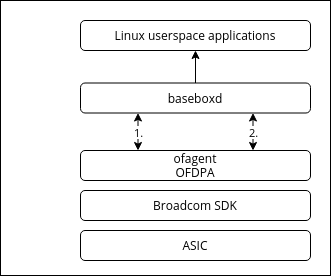
\includegraphics[scale=0.4]{baseboxd_architecture.png}
\caption{Basebox technology stack}
\end{figure}

\begin{enumerate}
\item main OpenFlow connection
\item gRPC connection, on-switch python daemon, used for tunnel configuration
\end{enumerate}

\end{frame}

\begin{frame}
\frametitle{So, how does Basebox work?}
\framesubtitle{OpenFlow}

\end{frame}

\begin{frame}
\frametitle{So, how does Basebox work?}
\framesubtitle{OF-DPA}
\begin{minipage}[t]{0.48\linewidth}
	%\includegraphics[scale=0.5]{OFDPAComponentLayers.jpg} 
	XXX include reference OpenFlow image, see OFDPAComponentLayers.jpg
\end{minipage}\hfill
\begin{minipage}[t]{0.48\linewidth}

   	OF-DPA is the application that translates OpenFlow messages into Broadcom SDK calls.
	
	OF-DPA abstracts:

	\begin{itemize}
	\item the network interfaces

	\item the ASIC hardware tables into constructs like flow and group tables
	\end{itemize}
\end{minipage}\hfill
\end{frame}

\begin{frame}
\frametitle{So, how does Basebox work?}
\framesubtitle{Netlink}

Netlink is Linux Kernel interface used for communication between user and kernel.

The Netlink socket family is referred to as AF\_NETLINK(AF: Address Family).

\end{frame}

\begin{frame}
\frametitle{So, how does Basebox work?}
\framesubtitle{Netlink}

Existing families in AF\_NETLINK like,

% [https://tools.ietf.org/html/rfc3549]
\begin{itemize}
\item NETLINK\_ROUTE: provides network interface status and routing information
\item NETLINK\_ARPD: provides an interface to the ARP table in the Linux Kernel
% NOTE: The number of netlink channels or ports (protocols) are limited to 32 [https://medium.com/@gilsonvarghese/generic-netlink-sockets-ceea20adb0bc]
\item NETLINK\_GENERIC: provides a generic family to extend the existing families (\#define MAX\_LINKS 32) % [https://elixir.bootlin.com/linux/v4.2/source/include/uapi/linux/netlink.h#L33]
\end{itemize}

\end{frame}

\begin{frame}
\frametitle{So, how does Basebox work?}
\framesubtitle{rtnetlink}

By binding to the NETLINK\_ROUTE socket we listen to the following messages:

{% Make table not overflow https://tex.stackexchange.com/a/423749 
\small
\visible<+->{

\begin{table}
\begin{tabular}{llll}
\hline 
Link & RTM\_NEWLINK & RTM\_GETLINK & RTM\_DELLINK \\ 
\hline 
Neighbors & RTM\_NEWNEIGH & RTM\_DELNEIGH & RTM\_GETNEIGH \\ 
\hline 
Route & RTM\_NEWROUTE & RTM\_DELROUTE & RTM\_GETROUTE \\ 
\hline 
Address & RTM\_NEWADDR & RTM\_DELADDR & RTM\_GETADDR \\ 
\hline 
\end{tabular} 
\end{table}
}}

\end{frame}

\begin{frame}
\frametitle{So, how does Basebox work?}
\framesubtitle{On Netlink messages}

% Describe serializing aspect, data types, and nested structures
\begin{minipage}[t]{0.48\linewidth}
\includegraphics[scale=0.4]{.png}
\caption{Basebox technology stack}

\end{minipage}

\end{frame}

\begin{frame}
\frametitle{So, how does Basebox work?}
\framesubtitle{Using rtnetlink}

% http://man7.org/linux/man-pages/man7/rtnetlink.7.html
% Link libnl

% build a specific Netlink message
% analyse return.

\end{frame}

\begin{frame}
\frametitle{So, how does Basebox work?}
\framesubtitle{Rule offload}

baseboxd then translates the information carried by the previously mentioned messages into the OpenFlow datamodel. 

Two OpenFlow help libraries known as rofl (Revised OpenFlow library).
\begin{itemize}
\item rofl-common: Core OpenFlow library, supporting versions from **check
\item rofl-ofdpa: library designed to work with the TableType Patterns present in the OFDPA implementation.
\end{itemize}
\end{frame}

\begin{frame}
\frametitle{So, how does Basebox work?}
\framesubtitle{Rule offload}

% Give specific examples on translating the model between netlink and OF
% Describe workflow for setting up interfaces, and such

\end{frame}

\begin{frame}
\frametitle{So, how does Basebox work?}
\framesubtitle{gRPC channel}

% VxLAN tunnels configuration is not well supported in OFPDA
%	How to enable VxLAN on OFDPA.
% Decision to implement separate channel to enable VxLAN on the switch
% Still necessary to bring up the Kernel version to support the feature

\end{frame}

\begin{frame}
\frametitle{So, how does Basebox work?}
\framesubtitle{code structure}

% Mention nl_l3 and cnetlink 
% Notable subsystems:
%	nl_bridge: handles bridge related stuff. Maybe point to vlan_aware bridge check in baseboxd!
%	XXX add

\end{frame}

\begin{frame}
\frametitle{So, how does Basebox work?}
\framesubtitle{L2 Bridging configuration}

\end{frame}

\begin{frame}
\frametitle{So, how does Basebox work?}
\framesubtitle{IPv6 Address configuration}

% RTM_NEWADDR notification
% handle message:
% 	1. Is loopback address? check interface flags
%		1.1 Add flow mod to table 30, match=IPv6 host / route address, destined to controller
%	2. Add termination MAC: handles decision to route or bridge the packets
%	3. Is link local address? yes, stop.
%	4. 

\end{frame}



\section{Further details}
\begin{frame}
\frametitle{So, how does Basebox work?}
\framesubtitle{Socket initialization}

\end{frame}



%\begin{frame}
%\frametitle{So, how does Basebox work?}
%\framesubtitle{IPv4 Address configuration}

%\end{frame}



\end{document}
